\documentclass[sigconf]{acmart}

%%
%% \BibTeX command to typeset BibTeX logo in the docs
\AtBeginDocument{%
  \providecommand\BibTeX{{%
    \normalfont B\kern-0.5em{\scshape i\kern-0.25em b}\kern-0.8em\TeX}}}

%%
%% end of the preamble, start of the body of the document source.
\begin{document}

%%
%% The "title" command has an optional parameter,
%% allowing the author to define a "short title" to be used in page headers.
\title{Amazon Fine Food Rating Prediction}

%%
%% The "author" command and its associated commands are used to define
%% the authors and their affiliations.
%% Of note is the shared affiliation of the first two authors, and the
%% "authornote" and "authornotemark" commands
%% used to denote shared contribution to the research.
\author{Weixin Li}
\email{wel006@ucsd.edu}
\affiliation{%
  \institution{A53286874}
}

\author{Weinan Li}
\email{w3li@ucsd.edu}
\affiliation{%
  \institution{A53264275}
}

\author{Jiacheng Hu}
\email{jih135@ucsd.edu}
\affiliation{%
  \institution{A91013815}
}


%%
%% The abstract is a short summary of the work to be presented in the
%% article.
\begin{abstract}
  In recent years with development of online shopping, more and more people tend to buy stuff online instead of going out to a real store. Amazon, as one of the biggest online shopping website, attracted huge amount of customers to its website. At this time, the recommender system plays an essential role in providing users with personalized recommendations. In this paper, we would like to build a recommender system to try to predict users’ ratings on products. We tried to build models based on the collaborative filter(KNN model) and the content-based filter(Proportional odds model). Initially the two models were trained and tested separately and then a hybrid model was build in order to optimize the performance. 
\end{abstract}

%%
%% Keywords. The author(s) should pick words that accurately describe
%% the work being presented. Separate the keywords with commas.
\keywords{Rating Prediction, Recommender systems, Collaborative Filtering, Content-based Filtering}

%%
%% This command processes the author and affiliation and title
%% information and builds the first part of the formatted document.
\maketitle

\section{Data set}
We use the Amazon Fine Food Reviews dataset:  \url{http://snap.stanford.edu/data/web-FineFoods.html}
\begin{itemize}
\item Number of reviews: 568,454
\item Number of users: 256,059
\item Number of products: 74,258
\item Time range: Oct 1999 - Oct 2012
\end{itemize}

\subsection{Basic Information}
This dataset contains the information in the following Table\ref{tab:dataset} 

\begin{table*}
  \centering
  \caption{Dataset basic description}
  \label{tab:dataset}
  \begin{tabular}{c|c|c}
    \toprule
    & Name & Description \\
    \midrule
    0 & Id: & Row ID\\
    1 & UserID: & Identifier for user\\
    2 & ProductID: & Identifier for product\\
    3 & ProfileName: & Profile name of the user\\
    4 & Time: & Timestamp for review\\
    5 & HelpfelnessDenominator: & Number of users who have voted for whether the review is helpful\\
    6 & HelpfulnessNumerator: & Number of users who have found the review is helpful\\
    7 & Score: & Rating from 1 to 5\\
    8 & Summary: & Brief summary of the review\\
    9 & Text: & Text of the review\\
  \bottomrule
\end{tabular}
\end{table*}

\subsection{Dataset Analysis}
\subsubsection{Relatinoship between Users and Items}
We looked into the dataset and tried to find out the frequency of items to be rated. As shown in the Fig \ref{1}, we found that the majority of items were rated only a few times, which means there’s not much connection between users and items for most of them. 
\begin{figure}
  \centering
  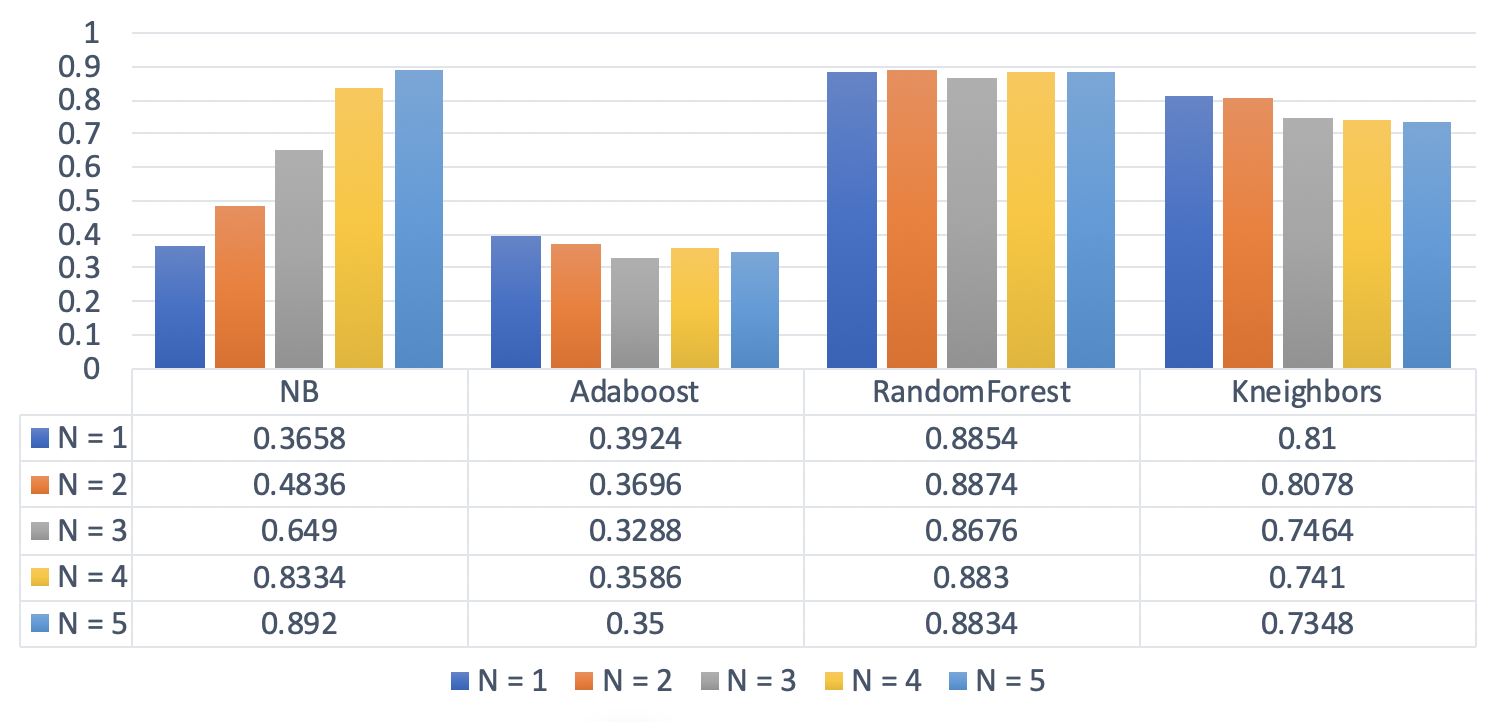
\includegraphics[width=2.5in]{4.png}
  \caption{Distribution of product rated by users}
  \label{1}
\end{figure}

\subsubsection{Rating Distribution}
For rating part, there are 568,454 ratings in this dataset. 363,122 (63.88\%) of them are 5-star, followed by 4-star(80,655/14.19\%), 1-star(52,268/9.19\%), 3-star(42,640/7.50\%) and 2-star(29,769/5.23\%). Result is shown in Fig \ref{2}. We found most of users are willing give the full rating score after their shopping.
\begin{figure}
  \centering
  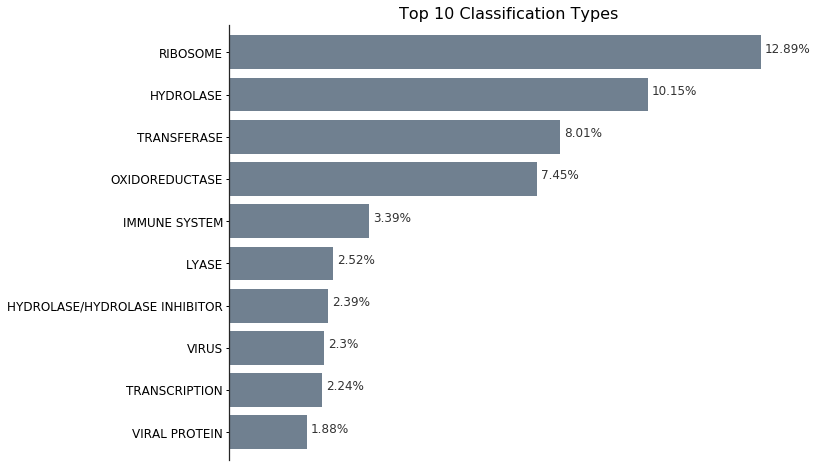
\includegraphics [width=2.5in]{3.png}
  \caption{Distribution of ratings}
  \label{2}
\end{figure}

\subsubsection{Sentiment Distribution}
For all the reviews, we set the reviews with ratings larger or equal to 4-star as positive reviews. 3-star reviews are set as neutral reviews.  All the other reviews are set as negative reviews. Result is shown in Fig \ref{3}. It also can reflect that most users are very satisfied with the product they bought.
\begin{figure}
  \centering
  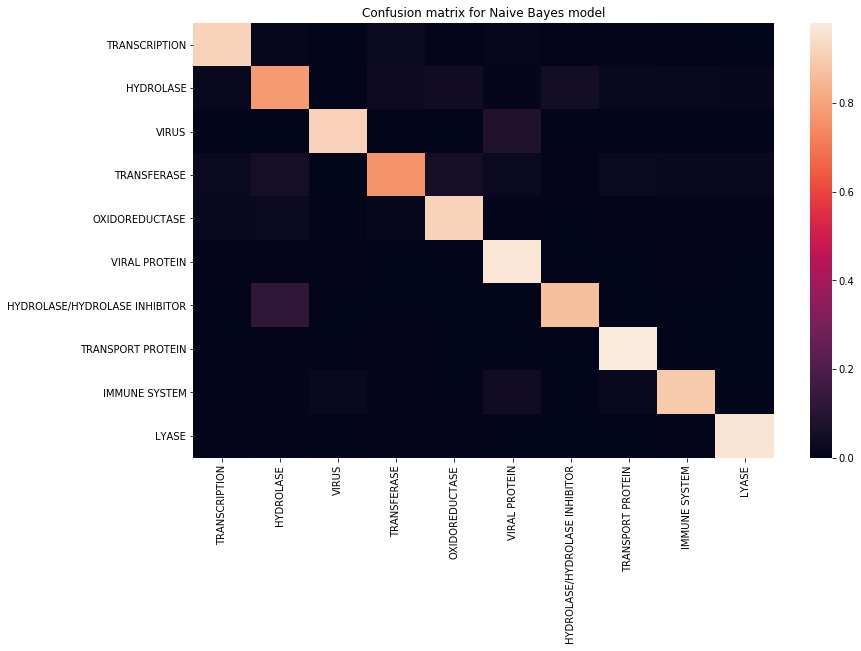
\includegraphics [width=2.5in]{5.png}
  \caption{Distribution of Review Sentiment}
  \label{3}
\end{figure}

\subsubsection{Word Clouds}
We gathered all existent words in the review. If we only wipe out punctuation, there are 38064 words. However, stop words like ”I”, ”a” don’t have many important meanings. If we erase them, this won’t affect the final result. After we remove English stop words, there are 37926 words now. In particular, we plotted top 100 common word clouds here: Fig \ref{4}. The more occurrences, the larger the word size.
\begin{figure}
  \centering
  \includegraphics [width=3.5in]{6.png}
  \caption{Top 100 Common Word Clouds}
  \label{4}
\end{figure}

\section{Predictive Task}
\subsection{Task Description}
Recommender systems, whose objective is to support users to make their choice. Our aim is to build an accurate recommender system based on our dataset so that given any pair of user and item we could predict a rating that the user would give. Based on that, we could also build personal recommendation ranking list for a user given later on but our priority is to accurately predict one's rating for a given item. We trained different models based on the training set and later on test on the test set.
\subsection{Evaluation Metric}
The most widely used evaluation metrics for recommender system are mean squared error (MSE)\cite{shani2011evaluating}. This evaluation metric result throughout the paper was calculated on a random test set that is of 10\% size of the whole dataset. We used this systems to check the performance of various models built. MSE is defined as:
\begin{equation}
    MSE = \frac{\sum(\hat{r}_{u, i} - r_{u, i})^2}{n}
\end{equation}
\subsection{Baseline}
Our baseline model is similar to the model used in [2]. A baseline estimate rating is denoted by $b_{u,i}$ and accounts for the user and item effects:
\begin{equation}
    b_{u,i} = \mu
\end{equation}
where $\mu$ is the mean rating of all reviews in the system. Here we ignore the differences of individual users, and simply predict from the overall rating score, we can imagine that this benchmark is very loose, but we think it still has reference value.

For each review in the dataset, we predicted the rating from the user to the business using the formula above and compared the prediction to the actual rating to calculate our baseline MSE. 

\section{Model}
Collaborative filtering and content-based filtering are the most common strategies to deal with the rating score prediction task\cite{si2004unified}. Here we proposed two different models that corresponded to two different filtering methods and continued to optimize each of the models from features selecting, model size, data filter conditions, etc. In the end, we tried to combine these two models to reach a better result.

\subsection{Collaborative filtering}
Collaborative filtering systems utilize the user’s past actions and relations to the other users to recommend goods\cite{si2004unified}. In general, this kind of system could be categorized into user-based and item-based and usually the item based one is more favorable due to the dynamic nature of users\cite{sarwar2001item}. From the observation of our dataset in previous section, a large number of users appeared only a few times in the dataset if not once. Hence, in our project, we applied item-based K-nearest neighbor model on the dataset. Another reason we did not adopt user-base KNN is that there’s too many users in the dataset and the majority of them rated only a few times and thus highly unpredictable. To deal with the problem and justify the characteristics of collaborative filtering systems, we also applied the model on dataset with different filter conditions.

In the K Nearest Neighbors model,  in order to predict the rating that user U would give to item I, we would like to know top k items that are similar to I and then calculate the weighted mean ratings from U on those k items. To find the similar items of U, we applied cosine similarity here as the single similarity measurement:

\begin{equation}
    sim(x, y) = cos(\theta) = \frac{\sum_{u\in U_{xy}}r_{u,x}*r_{u,y}}{\sqrt{\sum_{u \in U_{X}}r^2_{u,x}}*\sqrt{\sum_{u \in 
    U_{y}}r^2_{u,y}}}
\end{equation}

After received top k items that similar to I, we need to filter out the items that U has bought(rated) before. The final rating for the user-item pair given would be :

\begin{equation}
    r_{u,i} = \frac{\sum_{n\in N^k_u(i)}sim(i,n)*r_{u,n}}{\sum_{n\in N^k_u(i)}sim(i,n)}
\end{equation}

However, there’s a significant drawback in our approach with the original dataset due to the user rating frequency problem we previously mentioned. If a pair of user and item is come for rating prediction, it would be highly possible that we find top k items that are similar to our item but none of them were bought before by the user. Under this scenario, we’d have to give a prediction of global rating average or item rating average and this method is just the same as what we adopted in the baseline model. In order to evaluate  the performance of KNN algorithm, we filtered the dataset by the frequency of item rated. The filter condition P means only items rates time equals to or larger than P will be retained in the dataset.


\subsection{Content-based Filtering}
Content-based filtering predicts the rating score (1-5) from a user to a product by matching the user’s interests with a description and some attributes of the product. To create a comprehensive profile for users and products, we used raw numerical data from selected features in the user and product data. For the raw data input, we used 4 features for users:
\begin{itemize}
\item user average rating score
\item user average review count
\item user total review length
\item user average length per review
\end{itemize}
and used 4 features for products:
\begin{itemize}
\item product average rating score
\item product average review count
\item product total review length
\item product average length per review
\end{itemize}
To deal with the problem and justify the characteristics of content-based filtering, we also applied the model on the dataset with different filter conditions. (like using users who have more than 20 reviews, etc.)

We created our review matrix by replacing the user ID column with the user’s features, replacing the product ID column with product features. Ordinal multinomial logistic regression was applied to implement this approach.

\subsubsection{Ordinal Multinomial Logistic Regression (OMNLR)}

The review ratings we are trying to predict can take on a value  y $\in\{1,2,3,4,5\}$. Since these categories are ordered, we used a proportional-odds cumulative logit model to fit the data\cite{warner2008ordinal}. Assume the associated probabilities of each value y can take are $\{\pi_1,\pi_2, \pi_3, \pi_4, \pi_5 \}$ and the cumulative probability of y being less or equal to j is, 
\begin{equation}
    P(y\leq j)=\pi_1 + ... + \pi_j
\end{equation}
The proportional odd is, 
\begin{equation}
    L_j = ln(\frac{P(y\leq j)}{P(y > j)}) = ln(\frac{\pi_1+...\pi_j}{\pi_{j+1}+...+\pi_5})
\end{equation}
If we use covariates into the model and make the coefficient of each feature identical across the 4 logit equations, we have that 
\begin{equation}
    \begin{split}
    L_1 = \alpha_1 + \beta_1X_1 + ... + \beta_8X_8\\
    L_2 = \alpha_2 + \beta_1X_1 + ... + \beta_8X_8\\
    L_3 = \alpha_3 + \beta_1X_1 + ... + \beta_8X_8\\
    L_4 = \alpha_4 + \beta_1X_1 + ... + \beta_8X_8\\
    \end{split}
\end{equation}
Python package mold was applied to the training set to calculate the intercept terms α and coefficients $\beta$. Then $\alpha$ and $\beta$ were used to calculate the proportional odds of testing data. 

\subsection{Hybrid model(Optimized model)}
Since different filtering method has distinct advantages, we implemented a hybrid model to combine both content-based filter and collaborative filter, which can take the benefits of users’ and products’ features, while maintaining the advantages of a neighborhood model.\cite{leeprediction}

Specifically, we trained a KNN model first and obtained predictions for each users based on their neighbors. The prediction was then added to OMLR as a feature to recalculate the proportional odds model. 

We will discuss the strengths and weaknesses of the different models and different filter condition in the result and discussion part.

\section{Related Literature}
Currently the dataset we are using is a very authoritative and comprehensive dataset on Amazon food reviews.\emph{Julian McAuley. et al}'s work \cite{mcauley2013amateurs} directly using this dataset to predict the rating score given user-item pair. This paper introduced the level of experience, which builds an evolution model of user expertise through online review based on latent factor model. This model not only leads to better recommendations, but also allows us to study the role of user experience and expertise on a novel dataset of fifteen million beer, wine, food(the dataset we currently use), and movie reviews. 

Specifically for the fine food dataset, this model this paper proposed may get MSE 1.475  for total level, and the best single level MSE may get 0.960 (e = 5). On the other side, for our proposed combined filter model, the MSE can get 0.9611(p = 40), which is pretty close to the best result of the expertise model.

There are much more similar dataset for review & rating available in the website:  
\begin{itemize}
    \item BeerAdvocate reviews:
    
    \url{http://snap.stanford.edu/data/web-BeerAdvocate.html}
    \item RateBeer reviews:
    
    \url{http://snap.stanford.edu/data/web-RateBeer.html}
    \item CellarTracker reviews:
    
    \url{http://snap.stanford.edu/data/web-CellarTracker.html}
    \item Amazon reviews:
    
    \url{http://snap.stanford.edu/data/web-Amazon.html}
    \item Amazon movie reviews:
    
    \url{http://snap.stanford.edu/data/web-Movies.html}
\end{itemize}

We can directly use our proposed model in these datasets. Moreover, we found lots of state-of-the-art methods currently employed can study this type of data.

For instance, the Multinomial Naïve Bayes method\cite{panda2010discriminative} and Bernoulli Naïve Bayes method \cite{kim2006some} are applied in studying in this type of data. Comparing to the result of Combined model we proposed, the results from Multinomial Naïve Bayes method and Bernoulli Naïve Bayes method are less precise. 

In addition, in the field of Natural Language Processing, the dependency parsing is a method which can be used to find the grammar structure of sentences and the relationship between words \cite{cambria2014jumping}. This is a great direction for extracting new features We would like to continue to explore more features by NLP and apply these features into our proposed model in the future.

\section{Results and Conclusions}
\subsection{KNN Performance on different k}
Here we first present the results we achieved from the KNN model. We investigated the KNN model under numerous conditions changing the value of K.

\begin{figure}[h]
  \centering
  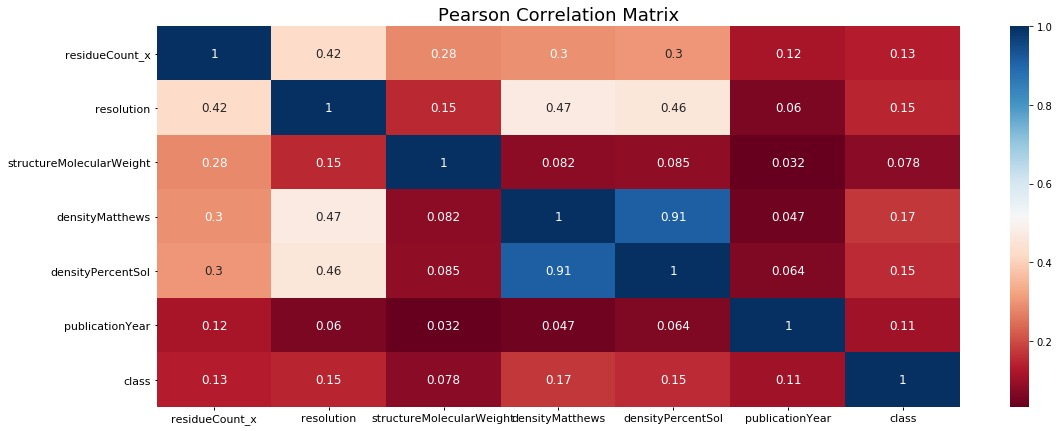
\includegraphics[width=\linewidth]{2.png}
  \caption{KNN Performance on different k}
  \Description{The 1907 Franklin Model D roadster.}
  \label{6}
\end{figure}

As shown in the Fig.\ref{6}. We explored the effect of the 'k' on the final performance based on filter condition P = 10 as shown in the figure below. Indeed, we could observe a declining MSE along with the increase of k. However, this decline is not as significant as previous dataset-filtering analysis.  We reached a consensus that the performance of the KNN model is highly dependent on the distribution dataset, the more sparse a dataset is, the worse KNN model performed. In a dataset of high sparsity as ours, the KNN model might not be the best option.

\begin{figure}[h]
  \centering
  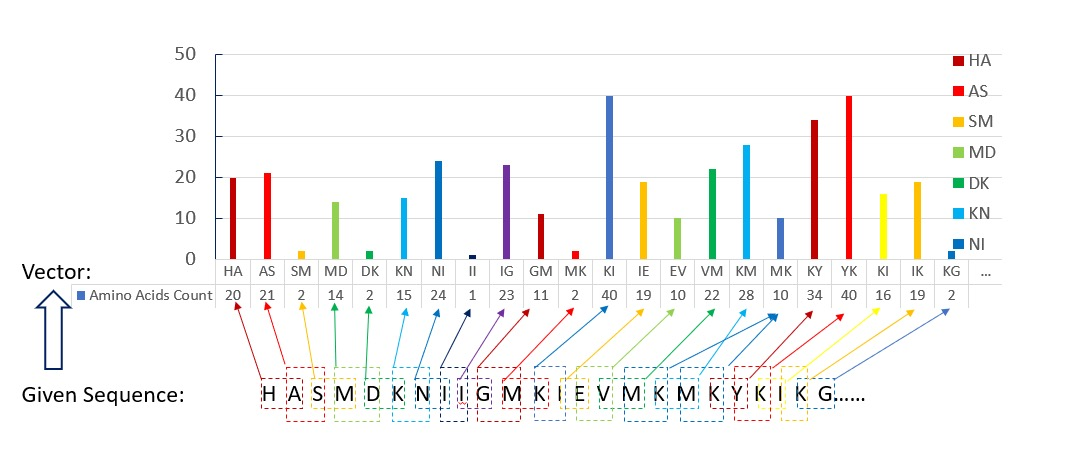
\includegraphics[width=\linewidth]{1.png}
  \caption{Model performance on different filter condition on the dataset}
  \Description{The 1907 Franklin Model D roadster.}
  \label{5}
\end{figure}

\subsection{Model performance on different filter conditions}
Then, we would like to discuss the model performance on different filter conditions on the dataset. As shown in the Fig.\ref{5}, with the increase of user-interaction (P) the performance of the models also boosted significantly. This fits our intuition that the more times that an item is bought the more predictive it will be. Also we can find that the proportional odds model perform better than KNN model on each filter conditions. 

\subsection{Final result comparison and analysis}
Next,we tried to use the rating given by the KNN model as a feature to feed in the regression model and see if this could give us better results. Here is a Table \ref{tab:res} to comparing different models which may suitable for this task.(80\% training set and 20 \% test set)

\begin{table}[h]
  \centering
  \caption{MSE of different suitable model for different filter conditions}
  \label{tab:res}
  \begin{tabular}{c|c|c|c}
    \toprule
    & Model & Filter condition = 0 & Filter condition = 40 \\
    \midrule
    0 & Baseline: & 1.6402 & 1.4711\\
    1 & KNN Model: & 1.6725 & 1.2309\\
    2 & OMNLR: & 1.4993 & 1.0650\\
    3 & OMNLR + KNN: & 1.4991 & 0.9611\\
  \bottomrule
\end{tabular}
\end{table}

From the MSE result table, we found that if we don't filter the items and take all the products into account, the combined model has hardly improved. We noticed that MSE of the KNN model without filter the products is much worse than the baseline. So that means the extra KNN feature can not give the OMNLR model more information it already got.

Fortunately, if we filter the products and only consider the products which have more than 40 reviews. The combined model has a better result than each of the single model. Because the filtered products have much information, and the KNN model can derive a valuable feature different than the other eight elements in the OMNLR model. This MSE is much better than the baseline's

\subsection{Parameter Interpretation}
Finally, let's focus on the coefficients of the combined model. This table 
\ref{tab:coef} shows the coefficients of the nine different features (p = 40):

\begin{table}[h]
  \centering
  \caption{MSE of different suitable model for different filter conditions}
  \label{tab:coef}
  \begin{tabular}{c|c|c}
    \toprule
    & Feature & Coefficients  \\
    \midrule
    1 & User average rating score: & 9.83697e-01 \\
    2 & User average review count: & 6.31897e-04\\
    3 & User total review length: & -1.19806e-06\\
    4 & User average length per review: & 6.23314e-06\\
    5 & Product average rating score& 1.56762e-01\\
    6 & Product average review count& -4.18116e-04\\
    7 & Product total review length& 2.21619e-06\\
    8 & Product average length per review& -2.59612e-04\\
    9 & KNN-derived feature & 5.77475e-03\\
  \bottomrule
\end{tabular}
\end{table}

We can find that the average rating is much higher than the others, which means the average rating plays the most crucial role. Also, the parameter of the feature derived from the KNN model larger than the other six parameters, which shows this feature influences much. Moreover, if we ignore the other six features, the final MSE may get worse, so we maintain every element in the combined model.

\subsection{Future Work}
We would like to analyze the review text and use this information to create more comprehensive user and product profiles. We would also want to explore more sophisticated hybrid techniques, such as cascade or switching methods.

\bibliographystyle{ACM-Reference-Format}
\bibliography{sample-base}
\end{document}
\endinput

